% Options for packages loaded elsewhere
\PassOptionsToPackage{unicode}{hyperref}
\PassOptionsToPackage{hyphens}{url}
%
\documentclass[
]{article}
\usepackage{lmodern}
\usepackage{amssymb,amsmath}
\usepackage{ifxetex,ifluatex}
\ifnum 0\ifxetex 1\fi\ifluatex 1\fi=0 % if pdftex
  \usepackage[T1]{fontenc}
  \usepackage[utf8]{inputenc}
  \usepackage{textcomp} % provide euro and other symbols
\else % if luatex or xetex
  \usepackage{unicode-math}
  \defaultfontfeatures{Scale=MatchLowercase}
  \defaultfontfeatures[\rmfamily]{Ligatures=TeX,Scale=1}
\fi
% Use upquote if available, for straight quotes in verbatim environments
\IfFileExists{upquote.sty}{\usepackage{upquote}}{}
\IfFileExists{microtype.sty}{% use microtype if available
  \usepackage[]{microtype}
  \UseMicrotypeSet[protrusion]{basicmath} % disable protrusion for tt fonts
}{}
\makeatletter
\@ifundefined{KOMAClassName}{% if non-KOMA class
  \IfFileExists{parskip.sty}{%
    \usepackage{parskip}
  }{% else
    \setlength{\parindent}{0pt}
    \setlength{\parskip}{6pt plus 2pt minus 1pt}}
}{% if KOMA class
  \KOMAoptions{parskip=half}}
\makeatother
\usepackage{xcolor}
\IfFileExists{xurl.sty}{\usepackage{xurl}}{} % add URL line breaks if available
\IfFileExists{bookmark.sty}{\usepackage{bookmark}}{\usepackage{hyperref}}
\hypersetup{
  pdftitle={Frontier : Geopolitical networks},
  pdfauthor={Claude Grasland},
  hidelinks,
  pdfcreator={LaTeX via pandoc}}
\urlstyle{same} % disable monospaced font for URLs
\usepackage[margin=1in]{geometry}
\usepackage{graphicx}
\makeatletter
\def\maxwidth{\ifdim\Gin@nat@width>\linewidth\linewidth\else\Gin@nat@width\fi}
\def\maxheight{\ifdim\Gin@nat@height>\textheight\textheight\else\Gin@nat@height\fi}
\makeatother
% Scale images if necessary, so that they will not overflow the page
% margins by default, and it is still possible to overwrite the defaults
% using explicit options in \includegraphics[width, height, ...]{}
\setkeys{Gin}{width=\maxwidth,height=\maxheight,keepaspectratio}
% Set default figure placement to htbp
\makeatletter
\def\fps@figure{htbp}
\makeatother
\setlength{\emergencystretch}{3em} % prevent overfull lines
\providecommand{\tightlist}{%
  \setlength{\itemsep}{0pt}\setlength{\parskip}{0pt}}
\setcounter{secnumdepth}{-\maxdimen} % remove section numbering
\usepackage{booktabs}
\usepackage{longtable}
\usepackage{array}
\usepackage{multirow}
\usepackage{wrapfig}
\usepackage{float}
\usepackage{colortbl}
\usepackage{pdflscape}
\usepackage{tabu}
\usepackage{threeparttable}
\usepackage{threeparttablex}
\usepackage[normalem]{ulem}
\usepackage{makecell}
\usepackage{xcolor}

\title{Frontier : Geopolitical networks}
\author{Claude Grasland}
\date{27/03/2021}

\begin{document}
\maketitle

\hypertarget{data-preparation}{%
\subsection{DATA PREPARATION}\label{data-preparation}}

\hypertarget{load-hypercube}{%
\subsubsection{Load hypercube}\label{load-hypercube}}

We have collected titles of news declared as \emph{international} as
long as we have depicted the existence of at less one foreign country in
the text of the title. In each of the 5 countries, we have selected
three newspapers with national audience and available through mediacloud
database from mid 2013 to mid 2020.

\hypertarget{load-geometrical-informations}{%
\subsubsection{Load geometrical
informations}\label{load-geometrical-informations}}

\hypertarget{international-networks}{%
\subsection{INTERNATIONAL NETWORKS}\label{international-networks}}

In this section, we propose to demonstrate the interest of an analysis
of triadic network of international relations which can be briefly
defined as the \emph{perception of the relation between two countries by
the media of another country}. In terms of cultural conflict, it is
indeed of utmost importance to take into account the role of \emph{third
party} which can be observer but also actors in the dynamic of opinion
at global scale. If we consider for example the crisis of Crimea, it is
typically an example of conflictual geopolitical link (between Ukraine
and Russia) which is perceived and reported differently in chinese,
indian or german newspapers. The same would be true for the geopolitical
links between Israel and Palestine, Northern and Southern Korea, USA and
Venezuela, etc.

But triadic network of international relation are not necessarily
related to conflicts and can also be simply associated to the production
of a perception of the geopolitical equilibrium of contemporary world.
Linkage between countries can indeed be related to sports, arts,
science, trade, \ldots{} But in every case they are not randomly
distributed across the world and the importance of the links depends
from the focus of the media which produce a localized vision of the
world.

\hypertarget{network-approach-of-foreign-news}{%
\subsubsection{Network approach of foreign
news}\label{network-approach-of-foreign-news}}

The method of co-quotation of countries has been firstly applied by
Segev (2010) on a large sample of 35 news sites collected between 1st of
February 2009 and 31st of July 2009. The objective of Segev was to
reveal the existence of different type of networks of international news
according to the place allocated to the host country where the media are
located. For this reason he did not exclude the links between the host
country and the other countries from the network of triadic relation.
And he demonstrated the existence of various types of networks of
foreign news illustrated by for examples :

\begin{itemize}
\tightlist
\item
  \emph{Self centered network} : like US newspapers where the majority
  of international links is related to the home country.
\item
  \emph{Global and regional networks} : like German newspapers where a
  dominant node is centered on the US but a secondary node on Germany in
  relation with more local relation in the EU
\item
  \emph{Two-hub networks} : like Russian newspapers where the network of
  international news is characterized by two cores of equal importance,
  US and Russia.
\item
  \emph{Regional network} : like Egyptian news where the network is not
  characterized by a dominant hub but by a mixture of countries of equal
  importance (Egypt, Israel, Palestina , USA, Syria, Lebanon)
\end{itemize}

\begin{figure}
\centering
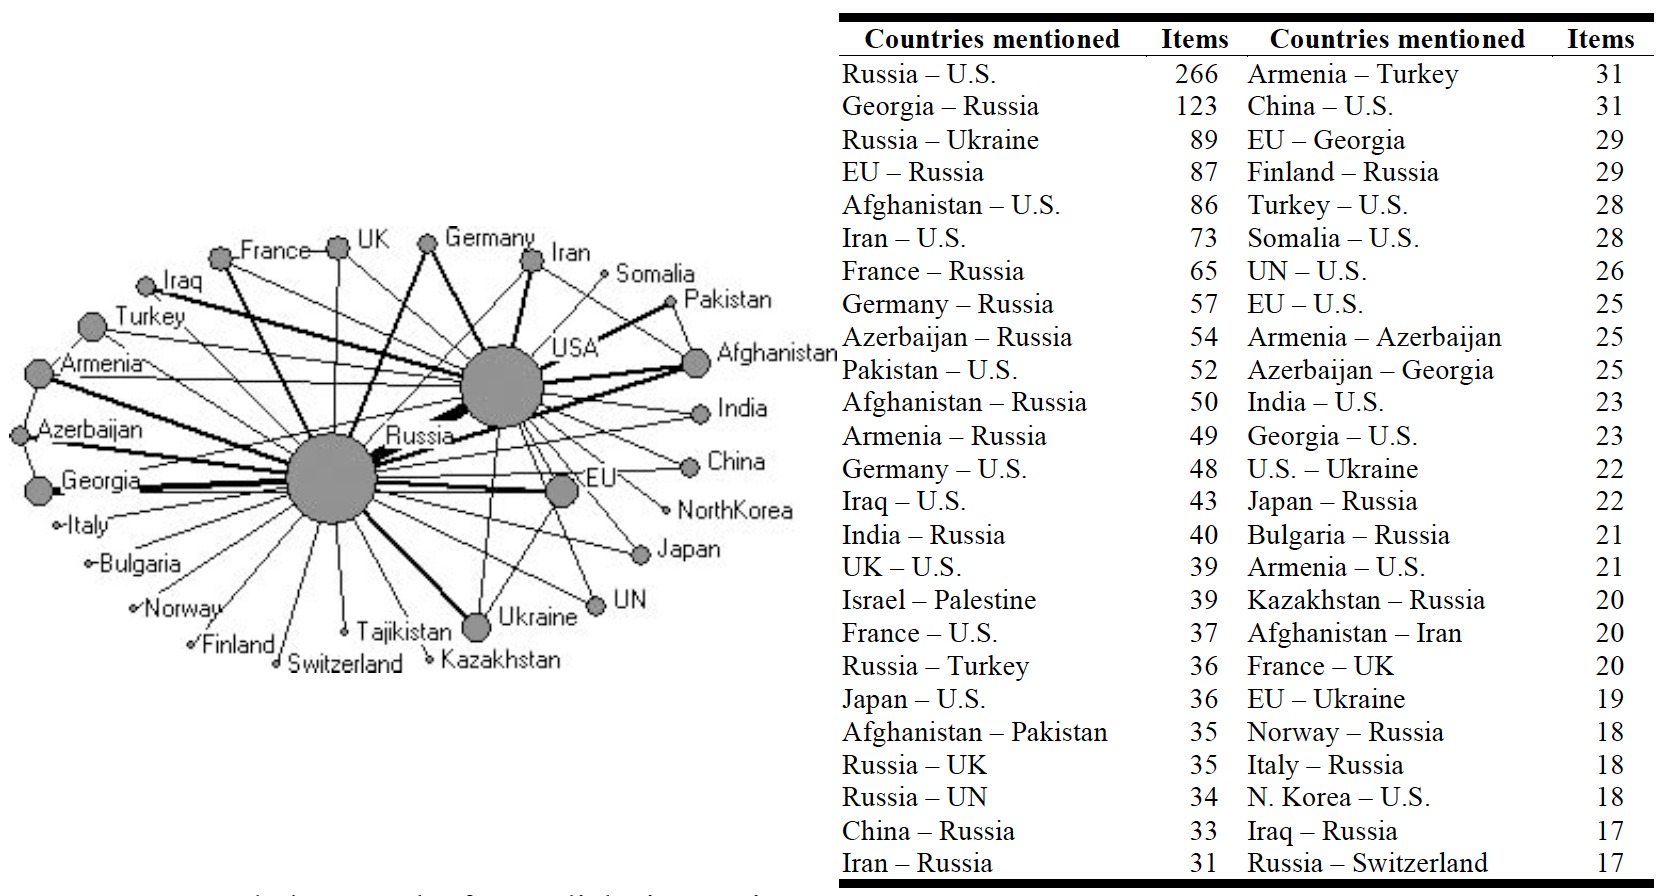
\includegraphics[width=0.9\textwidth,height=\textheight]{img/Segev2010a.png}
\caption{Association of countries in Russian news (Segev, 2010)}
\end{figure}

The analysis of co-occurence of countries in foreign news has been also
proposed by Grasland, Giraud \& Severo (2011,2016) in a paper about the
perception of Arab Spring in the title of news published by the
\emph{New York Time} and \emph{Liberation} between 11 May and 9 August
2011. In these case, the research focused on the linkages established by
media between countries located in eastern and southern Mediterranean
where the Arab Spring took place.

\begin{figure}
\centering
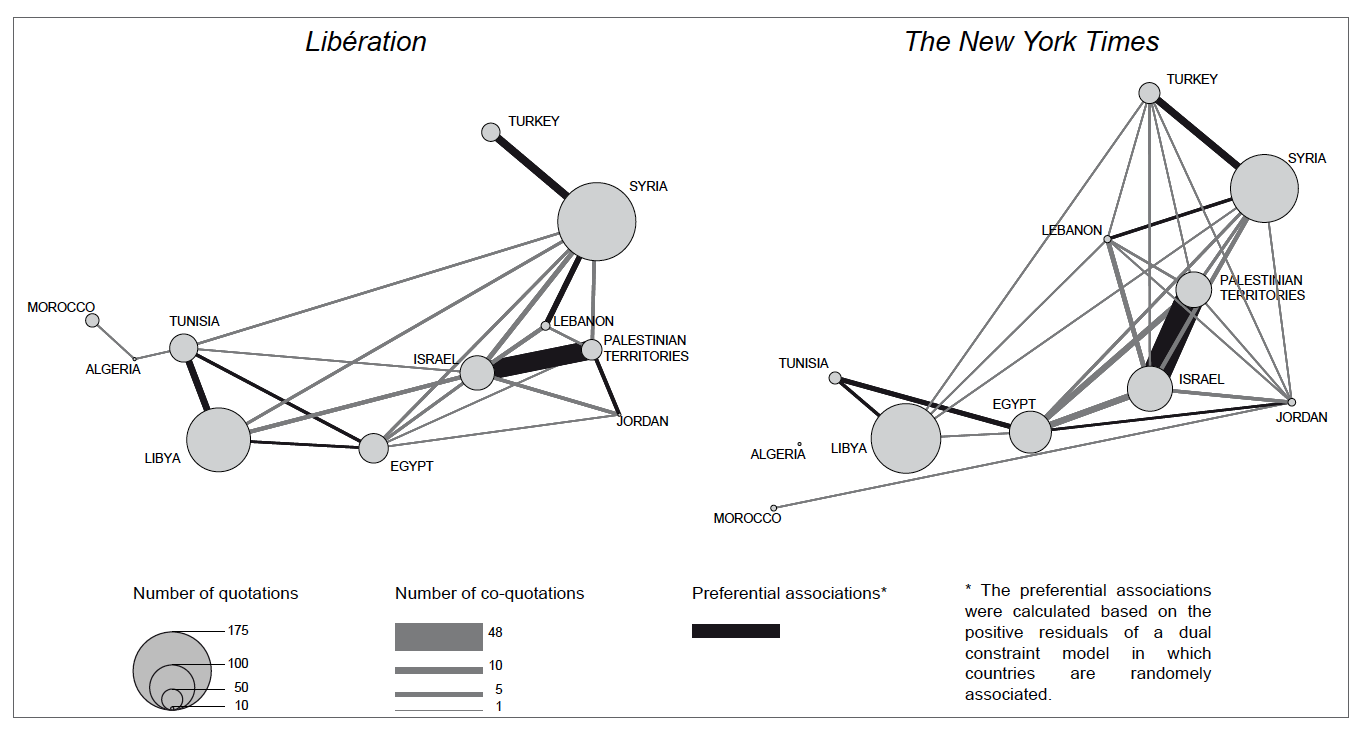
\includegraphics[width=0.9\textwidth,height=\textheight]{img/grasland_giraud_severo_2011.png}
\caption{The Arab Spring in French and US newspapers (Grasland, Severo
\& Giraud, 2011)}
\end{figure}

The authors demonstrated through this approach the existence of a
systemic perception of the geopolitcal transformation occuring in the
southern and eastern Mediterranean. But the analysis revealed also
different focus in the US and french newspaper. The network of the NYT
is more focused on the eastern part of the area with a major interest in
the case of the Israel-Palestin conflict but also in the Syrian civil
war. The network of the french newspaper Liberation is also focused on
the Israel-Palestin conflict but provide more attention to the Tunisia
and the other countries from Maghreb. This differences are in line with
geopolitical priorities which were not exactly the same for France and
USA during this period of time

\hypertarget{triadic-networks-of-international-relation}{%
\subsubsection{Triadic networks of international
relation}\label{triadic-networks-of-international-relation}}

The association of two countries in the news published by a media
located in another country can be used for the definition of
\textbf{triadic networks of international relation}.

\begin{itemize}
\tightlist
\item
  \(\mathcal{N}_{ij}^{m}\) : number of associations of countries i and j
  in the same sentences (title or description) of the news published by
  the media m from country k.
\end{itemize}

As we are focusing on international relation, we exclude the links
related to the country where the media is located. Contrary to Segev
(2010), we consider that it is difficult to decide when the country
where the media is located is present or absent from a news. In our
opinion, the host country of the media define \emph{first order dyads
(media form country k is speaking about foreiogn country i)} that should
not be confused with the \emph{second order triads (foreign countries i
and j are co-mentionned in news from media k)}. It is the reason why we
introduce the condition :

\begin{itemize}
\tightlist
\item
  \((i \neq k)\) and \((j \neq k)\)
\end{itemize}

It is possible to realize an aggregation of the triadic netwoks of
different media located in the same country :

\begin{itemize}
\tightlist
\item
  \(\mathcal{N}_{ij}^{k} = \sum_{m \in k } \mathcal{N}_{ij}^{m}\)
\end{itemize}

Or for a set of countries \(K = {k_1... k_n}\) like the five countries
of western Europe where our sample of media is located.

\begin{itemize}
\tightlist
\item
  \(\mathcal{N}_{ij}^{K} = \sum_{k \in K} \mathcal{N}_{ij}^{k}\)
\end{itemize}

But in this case we have to take into account the fact that
international relations of the set of countries \(K\) are partly
underestimated. In our example, the international links between France
and Germany can be reported by british, italian or spanish newspapers.
But not directly by french or german newspapers.

\hypertarget{top-linkages}{%
\subsubsection{Top linkages}\label{top-linkages}}

\begin{table}
\caption{\label{tab:unnamed-chunk-3}Top linkages for media from 5 western European countries (1st July 2013 to 30th June 2020}

\begin{tabular}[t]{r|l|r|r}
\hline
rnk & dyad & wgt & pct\\
\hline
1 & ISR-PSE & 4848 & 3.89\\
\hline
2 & RUS-UKR & 3786 & 3.03\\
\hline
3 & RUS-SYR & 2426 & 1.94\\
\hline
4 & CHN-USA & 2405 & 1.93\\
\hline
5 & RUS-USA & 2154 & 1.73\\
\hline
6 & SYR-TUR & 1954 & 1.57\\
\hline
7 & SYR-USA & 1315 & 1.05\\
\hline
8 & IRN-USA & 1309 & 1.05\\
\hline
9 & IRQ-SYR & 1292 & 1.04\\
\hline
10 & KOR-PRK & 1072 & 0.86\\
\hline
\end{tabular}
\begin{tabular}[t]{r|l|r|r}
\hline
rnk & dyad & wgt & pct\\
\hline
11 & PRK-USA & 1029 & 0.82\\
\hline
12 & DEU-FRA & 993 & 0.80\\
\hline
13 & MEX-USA & 958 & 0.77\\
\hline
14 & GBR-USA & 864 & 0.69\\
\hline
15 & CUB-USA & 776 & 0.62\\
\hline
16 & RUS-TUR & 683 & 0.55\\
\hline
17 & BEL-GBR & 678 & 0.54\\
\hline
18 & GBR-RUS & 669 & 0.54\\
\hline
19 & FRA-GBR & 657 & 0.53\\
\hline
20 & SAU-YEM & 654 & 0.52\\
\hline
\end{tabular}
\begin{tabular}[t]{r|l|r|r}
\hline
rnk & dyad & wgt & pct\\
\hline
21 & FRA-USA & 647 & 0.52\\
\hline
22 & DEU-GBR & 607 & 0.49\\
\hline
23 & BEL-FRA & 600 & 0.48\\
\hline
25 & CHN-RUS & 588 & 0.47\\
\hline
25 & DEU-USA & 588 & 0.47\\
\hline
25 & IRQ-USA & 588 & 0.47\\
\hline
27 & CHN-JPN & 571 & 0.46\\
\hline
28 & FRA-ITA & 556 & 0.45\\
\hline
29 & USA-VEN & 552 & 0.44\\
\hline
30 & DEU-GRC & 516 & 0.41\\
\hline
\end{tabular}
\end{table}

The top-20 linkages observed between countries for the 15 newspaper from
western Europe appears clearly as a perfect summary of the main
geopolitical conflicts and/or the struggle for power between the main
international actors during the period 2013-2020.

\begin{itemize}
\item
  \emph{Links related to precise conflicts and events} : At the top of
  the geopolitical agenda we can find the permanent issue of the
  Israel-Palestine conflict (rank 1), followed by the Russia-Ukraine
  conflict (rank 2) in relation with the annexion of Crimea in
  2014-2015. The war in Syria is also strongly present through links
  with Russia (rank 3), Turkey (rank 6) or USA (rank 7) or Iraq in
  relation with ISIS (rank 9). The Middle-East is also present through
  the conflicts between Iran and USA (rank 8), Russia and Turkey (rank
  16) or Saudi Arabia and Yemen (rank 20). Other links from this
  category are related to the relation between Northern and Southern
  Korea (rank 11), USA and Mexico about Trump's wall (rank 13) or USA
  and Cuba (rank 15).
\item
  \emph{Links related to structural relation between major power} : The
  list provide alos many examples of relations between major states of
  the world, that can not be assigned to precise events but rather to
  structural relations of power. This concern obviously the relations
  between USA and China (rank 4), USA and Russia (rank 5), Great Britain
  and Russia (rank 14). This structural relations are not necessarily
  related to negative oppositions and can also probably reveal linkages
  of friendship or collaboration like in the case of France and Germany
  (rank 12), France and UK (rank 19) or UK and USA (rank 14). The
  linkage observed between UK and Belgium (rank 17) is related to a
  false assignation of ``\emph{Bruxelles}'' to Belgium instead of
  European Union. It is in fact related to the Brexit crisis.
\end{itemize}

\hypertarget{geopolitical-variations-of-world-vision-in-western-europe}{%
\subsubsection{Geopolitical variations of world vision in western
Europe}\label{geopolitical-variations-of-world-vision-in-western-europe}}

Do we observe the same distribution of gopolitical priorities in the
newspapers of five countries of western Europe ? To answer the question
we compute the top geopolitical links for each country, but with the
exclusion of the five countries themselves.

\begin{table}

\caption{\label{tab:unnamed-chunk-4}Variation of top international dyads by host country}
\centering
\begin{tabular}[t]{l|l|l|l|l|l}
\hline
  & Germany & Spain & France & U.K. & Italy\\
\hline
1 & RUS-UKR & ISR-PSE & ISR-PSE & ISR-PSE & ISR-PSE\\
\hline
2 & CHN-USA & RUS-UKR & RUS-UKR & RUS-UKR & CHN-USA\\
\hline
3 & RUS-USA & RUS-USA & RUS-SYR & RUS-SYR & RUS-UKR\\
\hline
4 & RUS-SYR & CHN-USA & CHN-USA & SYR-TUR & RUS-USA\\
\hline
5 & SYR-TUR & MEX-USA & SYR-TUR & AUS-NZL & RUS-SYR\\
\hline
6 & ISR-PSE & CUB-USA & RUS-USA & SAU-YEM & SYR-TUR\\
\hline
7 & IRN-USA & USA-VEN & IRN-USA & IRQ-SYR & SYR-USA\\
\hline
8 & SYR-USA & SYR-USA & SYR-USA & KOR-PRK & IRQ-SYR\\
\hline
9 & PRK-USA & RUS-SYR & IRQ-SYR & RUS-USA & CHN-JPN\\
\hline
10 & IRQ-SYR & IRN-USA & KOR-PRK & AUS-IND & CHN-RUS\\
\hline
11 & KOR-PRK & PRK-USA & PRK-USA & CHN-USA & PRK-USA\\
\hline
12 & RUS-TUR & IRQ-SYR & MEX-USA & IND-PAK & BRA-RUS\\
\hline
13 & TUR-USA & COL-VEN & RUS-TUR & IRL-NZL & BEL-SRB\\
\hline
14 & MEX-USA & SYR-TUR & SAU-YEM & CHN-PRK & RUS-TUR\\
\hline
15 & CHN-RUS & KOR-PRK & CAN-USA & IRN-USA & ISR-SYR\\
\hline
16 & GRC-TUR & IRQ-USA & ISR-USA & PRK-USA & MEX-USA\\
\hline
17 & IRN-ISR & JPN-USA & CUB-USA & CHN-RUS & IRQ-USA\\
\hline
18 & CHN-PRK & CAN-USA & ISR-SYR & AUS-ZAF & IRN-USA\\
\hline
19 & CHN-JPN & ISR-USA & CHN-JPN & SYR-USA & CUB-USA\\
\hline
20 & CUB-USA & AFG-USA & IRN-ISR & RUS-TUR & JPN-USA\\
\hline
\end{tabular}
\end{table}

The analysis of the variation of the top international by country of
localization of the media reveals a global stability of the pattern of
the top-10 couples of foreign countries mentioned. But some interesting
variations can be pointed which reveals different focus, different
visions of the world.

\begin{itemize}
\tightlist
\item
  The \emph{Israel-Palestin} conflict appears in first rank of dyads
  mentionned in all countries, with the exception of Germany where it
  appears only in 6th rank. If this difference is not related to a
  problem in the dictionary of countries (\textbf{to be verified}) it
  reveals a real originality of German newspapers as compared to the
  rest of western Europe?
\item
  The \emph{Russia-Ukraine} dyad appears in first rank in Germany, in
  second rank in Spain, France and UK and in third rank in Italy. It is
  therefore the most consensual topic of geopolitical interest of our
  sample.
\item
  \emph{Specific dyads} appears in the top-10 of countries, in relation
  with cultural proximities inherited from history and related to
  language or former colonial relations. It is typically the case of the
  dyads linking Australia and New-Zealand or Australia and India in UK
  newspapers. Or the high level of the dyads USA-Mexico and USA-Cuba in
  the case of spanish newspapers. Or the link between Greece and Turkey
  in German newspapers, etc.
\end{itemize}

\hypertarget{spatial-network}{%
\subsection{SPATIAL NETWORK}\label{spatial-network}}

How to propose a spatialization of the networks previously described ?
We propose in a first step a version of the global network based on
intensity and transparency, like the famous Facebook global connexion
map realized by Paul Butler in 2010.

\begin{figure}
\centering
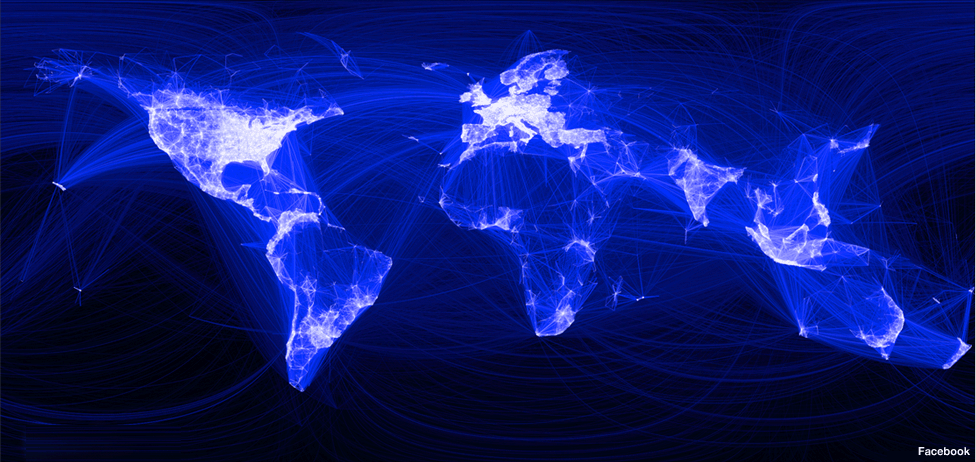
\includegraphics[width=0.7\textwidth,height=\textheight]{img/facebook_butler_map.png}
\caption{Facebook Global Connexion Map (Butler, 2010)}
\end{figure}

\begin{figure}
\centering
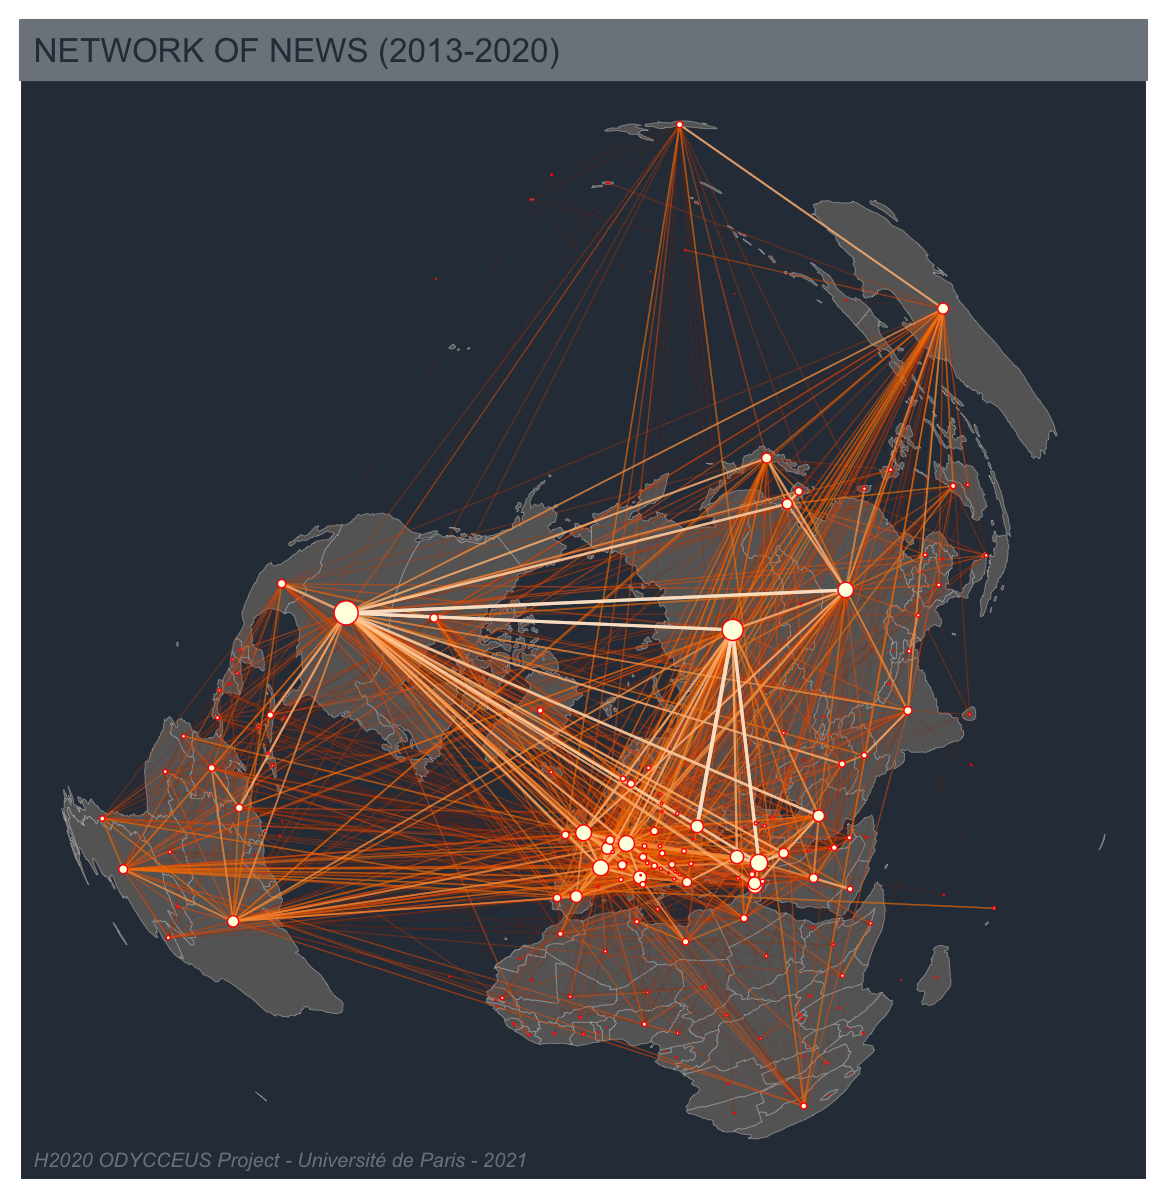
\includegraphics[width=0.9\textwidth,height=\textheight]{img/News_global.png}
\caption{Network of international news}
\end{figure}

The network of news appears clearly dominated by major world power
(Russia, Usa, China, Japan, France, Germany and UK) but also by major
conflicts occuring in the period (Ukraine, Syria, Northern Korea, Iran,
\ldots). The Middle East appears as an area of central interest for our
sample of media from western Europe. Latin America is also relatively
well connected, thanks to the focus of spanish newspapers and the
olympic games of 2016 held in Brazil. But the most striking fact is the
lack of interest for the majority of african countries, except the
northern part and the RSA. Th same is true to some extent for south
eastern Asia countries which are very few mentionned, except by british
newspapers. We have of course to notice that these map of dyad focus on
the countries that are associated with other in the news. Therefore, the
countries that are mentioned alone in news are less visible. Biut the
fact to be isolated is precisely an evidence of marginal situation in
the vision of the world produce by European newspapers.

\hypertarget{dominant-network}{%
\subsection{DOMINANT NETWORK}\label{dominant-network}}

The distribution of dyads over a long period of time and for a large set
of newspapers offers the possibility to establish an international
network of relation which can reveal structural position of countries
according to a hierarchy of dominant, intermediary and dominated
countries. To establish this hierarchy, we use the method of
\emph{dominant flows} initially developped by John D. Nyusten \& Michael
F. Dacey (1961) for the delineation of nodal regions based on a graph of
tecommunication flows between cities. Considering a matrix of weigthed
dyads between countries \(\mathcal{N}_{ij}\), the authors consider that
a country \(i\) is dominated by a country \(j\) if two conditions are
verified :

\begin{itemize}
\item
  \textbf{Condition 1} : The most important association of country i is
  with country j : \(max_{z}(\mathcal{N}_{iz}) = \mathcal{N}_{ij}\)
\item
  \textbf{Condition 2} : The sum of association of country i with other
  coutries is lower than the one of country j :
  \(\sum_{z} \mathcal{N}_{iz} < \sum_{z} \mathcal{N}_{jz}\)
\end{itemize}

For example, the country which is the most associated with China in our
sample of newspaper is the USA (\(\mathcal{N}_{ij} = 1202\)) and the sum
of association of USA with other countries
(\(\mathcal{N}_{j.} = 10807\)) is larger than the sum of associations of
China with other countries(\(\mathcal{N}_{i.} = 4486\)). Therefore China
is ``dominated'' by USA according to the model of Nyusten \& Dacey.

In the case of Australia, the most associated country is New-Zealand
(\(\mathcal{N}_{ij} = 227\)) but the sum of association of New-Zealand
with other countries (\(\mathcal{N}_{j.} = 747\)) is lower than the sum
of associations of Australia (\(\mathcal{N}_{i.} = 2256\)). In this
case, the theory conclude that Australia is not dominated anc can be
consider as the core of a network of countries. The application of the
method to all countries of the world define a graph which is organised
as a set of trees with core countries as center of each component of the
graph. Countries can be classified in three basic types according to
their position in the trees

\begin{enumerate}
\def\labelenumi{\arabic{enumi}.}
\tightlist
\item
  \textbf{Roots} are dominant countries, represented in red
\item
  \textbf{Nodes} are countries which are at the same time dominant ane
  dominated, represented in orange.
\item
  \textbf{Leaf} are countries which are purely dominated, represented in
  yellow.
\end{enumerate}

The advantage of the method is to produce a simplified but very clear
divsion of the network in hierarchical regions centered on a dominant
geopolitical actor. The application to our sample of western European
newspapers for the period 2013-2020 produce an exciting picture of the
world seen by media.

\begin{figure}
\centering
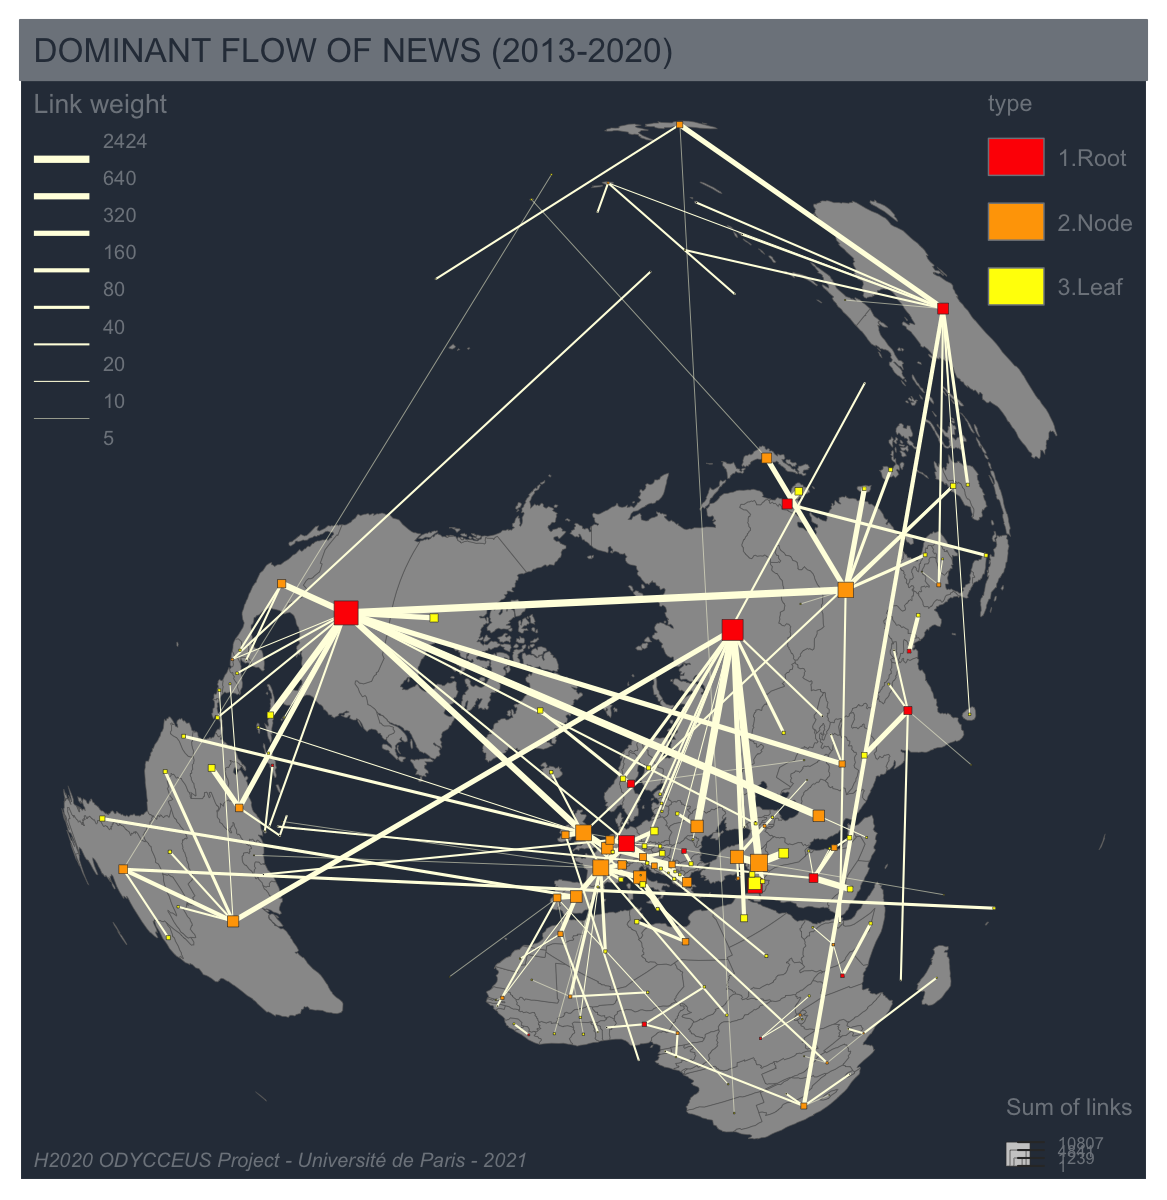
\includegraphics[width=0.9\textwidth,height=\textheight]{img/DomNews_global.png}
\caption{Dominant flows in international news}
\end{figure}

The map reveals firstly the existence of four global networks which take
the form of giant trees centered respectively on USA, Russia , European
Union and Australia

\begin{itemize}
\item
  \textbf{The American network} is the largest one. It is firstly
  centered on countries from northern and central America, wich are
  directly dominated by USA or indirectly through the branchs of Mexico
  and Venezuela. The network is extended to south-eastern Asia through
  the major branch of China which dominates Japan, Taiwan, Phlipinnes,
  \ldots{} The ``special relation'' between USA and Great Britain is
  confirmed by another branch across the northern atlantic but with few
  secondary connections in EU, except Ireland. Last but not least,
  important links are observed between USA and Iran or Afghanistan,
  which is clearly in line with the geopoilitical implication of USA in
  this countries during the period. But we do not observe dominant links
  with the rest of Middle-East where the network structure reveals the
  role of other major players?
\item
  \textbf{The Russian network} covers firstly countries from former
  Soviet Union, Central Asia and Middle East, with very important
  linkages with Ukraine on the one hand, Syria and Turkey on the other
  hand, followed by secondqry links with Iraq, Lebanon or Jordan. The
  impôrtance of the Russian network has clearly grown during the last
  years and was less important in the previous work realized by Elad
  Segev in 2009. Without any doubt, the geopolitical activism of Russia
  is reflected by the media. More suprinsingly, Russia appears also
  strongly connected with Brazil which is a relay for the southern part
  of Latin America. The explanation of this linkage is probably to be
  found to the events of the Olympic Games of 2016 in Brazil where
  Russia was initially excluded and finally accepted.
\item
  \textbf{The European Union network} is organized around the dual core
  of France and Germany which are characterized by a strong reciprocal
  link (497) and and equivalent number of external dyads (4683 and
  4784). The strict application of the model of Nyusten \& Dacey which
  would implies a domination of France by Germany should be relaxed
  considering the small différence of size and it is more relevant to
  consider both countries as a common backbone. Each of the two core
  countries organize a specific sub-tree. France network covers
  south-western Europe and northern Africa with important sub-branch in
  Spain and Italy. Germany netwok is more oriented toward eastern
  Europe, with major sub-branch in Austria or Greece.
\item
  \textbf{The Australian network} plays clearly a major role in Oceania
  but also southern Africa and south eastern Asia. Two important
  secondary branchs take place in New Zealand and RSA. The importance of
  this Australian network does not necessarily fit with a real
  domination of the country in terms of hard power. It is rather a
  reflect of the smart power of Australia in the eyes of newspapers from
  Western Europe and - in particular - british newspapers which are
  stro,ngly connected to australian newspapers by financial ties (Cf.
  Murdoch empire).
\end{itemize}

Out of this four giant components, we can observe more regional or local
networks that are generally based on the existence of couples of
strongly connected countries like Israel and Palestin, Northern and
Southern Korea, India and Pakistan, Saudi Arabia and Yemen, Sweden and
Denmark\ldots{}

\end{document}
